% Created 2023-05-20 周六 09:24
% Intended LaTeX compiler: pdflatex
\documentclass[lang=cn,12pt,bibtex,newtx,twoside,margintrue,citestyle=gb7714-2015, bibstyle=gb7714-2015]{elegantbook}
\usepackage[utf8]{inputenc}
\usepackage[T1]{fontenc}
\usepackage{graphicx}
\usepackage{longtable}
\usepackage{wrapfig}
\usepackage{rotating}
\usepackage[normalem]{ulem}
\usepackage{amsmath}
\usepackage{amssymb}
\usepackage{capt-of}
\usepackage{hyperref}
\cover{cover1.jpg}
\logo{logonpu.pdf}
\graphicspath{{./figure/}}
\usepackage{svg,subcaption,caption,threeparttable}
\usepackage{bicaption}
\captionsetup[table][bi-second]{name=Table}
\captionsetup[figure][bi-second]{name=Figure}
\addbibresource{reference.bib}
\author{刘望奇 2022261571}
\date{\today}
\title{智能制造}
\hypersetup{
 pdfauthor={刘望奇 2022261571},
 pdftitle={智能制造},
 pdfkeywords={},
 pdfsubject={},
 pdfcreator={Emacs 28.2 (Org mode 9.5.5)}, 
 pdflang={English}}
\begin{document}

\maketitle
\tableofcontents

\mainmatter

\chapter{智能制造}
\label{sec:org0099496}
\section{智能制造概述}
\label{sec:org855a6fd}
\subsection{智能制造的定义和特征}
\label{sec:org9982659}

关于智能制造的定义,目前不同国家在表述上有一些差异。在工信部发布的《智能制造发展规划(2016-2020年)》中给出了智能制造一个新的表述:“智能制造是基于新一代信息通信技术与先进制造技术深度融合,贯穿于设计、生产、管理、服务等制造活动的各个环节,具有自感知、自学习、自决策、自执行、自适应等功能的新型生产方式。”\cite{01}

总的来说,智能制造是一种基于现代信息技术的高度自动化、智能化和网络化的制造模式,旨在通过整合物理系统、数字系统和智能系统,实现制造过程的高效、灵活、可持续和个性化。智能制造技术英文名称是Intelligent Manufacturing,其主要是指以新兴科技为依托,配合新工艺、新能源以及新材料等综合生产、管理以及服务等各个要素进行智慧化集成,精确控制各个模块,将功能实现智能化的总称\cite{02}。

智能制造主要包含以下几个特征:

自动化和智能化。智能制造利用先进的自动化技术和智能算法,实现生产过程的自动化和智能化,减少人为干预,提高生产效率和质量。

数据驱动和信息化。智能制造通过大数据、云计算、物联网等技术,实现对制造过程中产生的海量数据的采集、分析和利用,以实现更好的决策和优化。

灵活性和个性化。智能制造具有快速响应市场需求、灵活调整生产线和产品配置的能力,能够实现批量定制和个性化生产,满足消费者多样化的需求。

协同和互联。智能制造通过网络连接不同的生产设备、系统和供应链的各个环节,实现信息共享、协同操作和实时反馈,提高资源利用效率和生产协调能力。

可持续和绿色。智能制造注重资源的高效利用和环境的保护,通过优化生产过程、减少能源消耗和废弃物排放,实现可持续的生产模式和绿色制造。

\subsection{智能制造的发展历程}
\label{sec:org97670eb}
人类的历史永远没有离开过制造业,制造活动是人类进化生存和生产活动中的一个永恒主题,是人类建立物质文明和精神文明的基础。与工业化进程和产业革命紧密相联,制造业先后已经历了机械化、电气化和信息化三个阶段,现在正处于智能化发展的第四个阶段,这四个阶段现在普遍被称为四次工业革命(分别称为工业1.0、工业2.0、工业3.0和工业4.0),如图\ref{1.1}所示。

\begin{figure}[htbp]
\centering
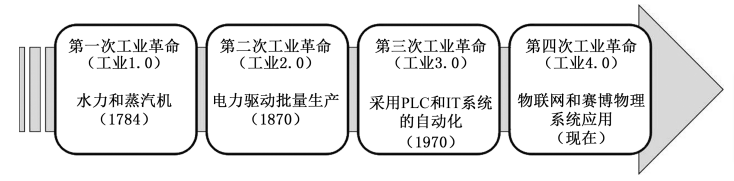
\includegraphics[angle=0,width=10cm]{./figure/1.1.png}
\caption{\label{1.1}四次工业革命}
\end{figure}

第一次工业革命的主要标志是蒸汽机和动力的使用,将人类带入了蒸汽时代。此时的生产模式还是单件小批量生产,但是可以使用基本的机械结构代替一定的人力,形成了集中动力源的机床。第一次工业革命解决了“人力效率低下和动能不足的问题”。

第二次工业革命是以发电机为代表的“电力时代”。1831年法拉第发明了世界上第一台发电机。1866年德国人西门子制成世界上第一台工业用发电机,标志着电力开始在工业生产中大规模应用。第二次工业革命解决了“规模化和生产成本之间的矛盾”。

第三次工业革命是以计算机为代表的“信息时代”。从1946年美国发明第一台计算机开始,直到当今互联网时代,人类信息化一直在加快,并未结束。第三次工业革命实现了“解放人的体力劳动和替代部分脑力劳动”。

第四次工业革命是实虚融合的“数字时代”,以2012年美国GE公司发布“工业互联网”、2013年德国提出“工业4.0”、2015年中国提出“中国制造2025”为标志。第四次工业革命的驱动力是从客户个性化需求出发,定制化的生产技术、复杂的流程管理、庞大的数据分析、决策过程的优化、行动的快速执行构成了第四次工业革命的主体。

\begin{figure}[htbp]
\centering
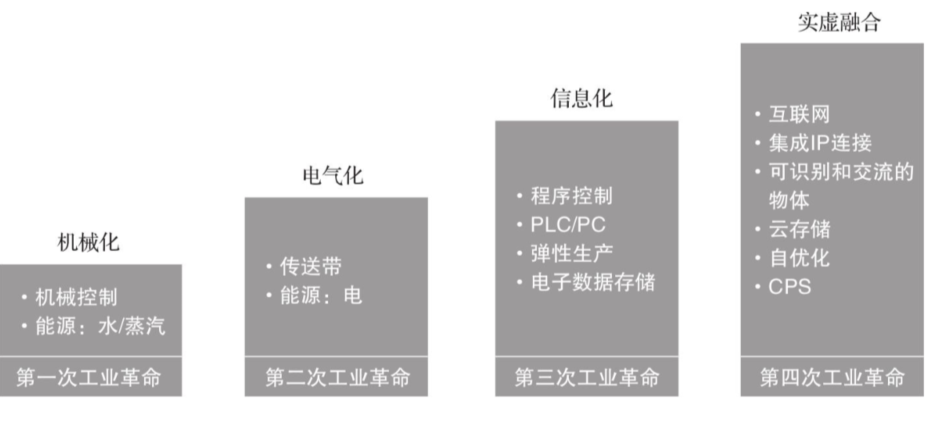
\includegraphics[angle=0,width=10cm]{./figure/1.2.png}
\caption{\label{1.2}人类历史上四次工业革命带来的变化与新技术}
\end{figure}

智能制造的提出是在第三次工业革命之后。20世纪80年代,智能制造的概念第一次被提出,旨在通过集成专家知识库、机器人控制系统来对制造过程进行建模,达到使机器可以智能自主生产的目的,标志着智能制造进入了数字制造阶段,由人类专家知识库与机控软件和硬件集成的数字制造系统可以代替人类完成各种任务。

到20世纪末,快速发展的互联网和其广泛的连接支持使其被应用在各行业,网络系统的引入是智能制造一次大的发展。在网络系统支持下,各要素包括人员和物理设备等都连接在一起,标志着智能制造进入数字网络制造阶段。工业互联网和云平台的提出,使之成为网络系统与物理系统集成的关键组件,为智能制造的发展再一次提供了源源不断的动力。

日新月异的新型信息技术使得智能制造迈入了新一代智能制造阶段,数字孪生为制造活动提供物理世界的完美虚拟映射。机器学习学习人类专家知识,并抓取制造数据,建立更完全的数据库不断优化制造过程。边缘计算提供边缘计算资源支持和缓存服务。


\subsection{智能制造的体系架构}
\label{sec:orgc946446}
不同的智能制造系统可能会有不同的架构体系,但是通常包含以下一些核心部分。

设备层,指生产过程中的各种物理设备,包括机械设备、传感器、执行器等。这些设备通过物联网技术连接到网络中,实现数据的采集和传输。

数据层,是指智能制造中产生的各种数据,包括生产数据、传感器数据、监测数据等。这些数据通过传感器、控制系统等设备进行采集,并通过网络传输到数据中心进行存储和处理。

控制层,智能制造的核心,负责对生产过程进行实时监控和控制。通过对数据的分析和处理,控制层能够对生产过程进行调整和优化,实现智能化的生产控制。

决策层,基于数据和控制层的分析结果,进行生产决策和调度。这包括生产计划的制定、资源调度、任务分配等。决策层可以根据实时数据和预测模型进行智能化决策,实现生产过程的优化和灵活性。

服务层,为智能制造提供支持和服务,包括设备维护、远程监控、故障诊断、用户服务等。通过服务层的支持,能够确保智能制造系统的稳定运行和及时维护。

安全层,用于保障智能制造系统安全性和可靠性,包括网络安全、数据隐私、设备安全等。智能制造系统涉及大量的数据和网络连接,安全层的存在能够有效防范安全威胁和风险。

这些层之间通过网络连接和数据交换实现信息的传递和协同工作,形成一个完整的智能制造体系架构。不同的智能制造体系架构可能有所差异,但核心的层次和功能一般是类似的,以实现生产过程的智能化、高效化和灵活化为目标。

\subsection{智能制造的未来发展趋势}
\label{sec:orgf00b0f0}
美国未来学家托夫勒在1980年出版的《第三次浪潮》一书中\cite{托夫勒2006},预测了未来的工业生产方式具有以下的特征:小规模、定制化;在大城市以外的地方工业生产与日俱增;利用更少的能源,消耗更少的原料,使用更少的零部件,以及要求更多的智能设计;工厂的许多机器由消费者直接远程操作而不是由工人来操作。

其中我们大致也可以看到一些未来的智能制造发展趋势:首先,人工智能和机器学习技术将在智能制造中发挥更重要的作用。通过数据分析和机器学习算法,智能制造系统能够自动学习和优化生产过程,提高生产效率和质量。同时云计算和大数据技术的发展将为智能制造提供更强大的数据处理和存储能力。通过将数据存储在云端,并利用大数据分析技术,可以实现对庞大数据量的高效处理和智能决策。

其次,物联网和传感器技术的进一步发展将实现更广泛的设备连接和数据采集。智能制造系统可以通过物联网连接各种设备,并通过传感器实时获取生产数据,实现设备之间的协同工作和智能控制。自动化和机器人技术在智能制造中的应用将进一步扩大。自动化系统和机器人能够完成更复杂的生产任务,提高生产效率和灵活性。智能制造将推动供应链的数字化和智能化。通过信息技术和物联网的应用,可以实现供应链的实时可视化和智能协调,提高供应链的效率和响应速度。

最后,智能制造将越来越多地融合其他领域的创新技术,如生物技术、纳米技术、新材料等。这种跨领域融合将推动智能制造的发展,开辟更多的应用领域和商业机会。智能制造将越来越注重可持续发展和绿色制造的理念。通过优化生产过程和资源利用,减少能耗和环境影响,实现可持续发展和绿色制造。

\section{智能制造核心技术}
\label{sec:org6b50d0a}
\subsection{智能传感技术}
\label{sec:org708845b}
物联网(Internet of Things, IoT)和传感器技术在智能制造中起着重要的作用。它们使得设备、系统和人员能够互相连接和交换数据,实现智能化的生产和管理。

物联网是指将各种物理设备、传感器、执行器和计算机系统通过互联网进行连接和通信的网络。在智能制造中,物联网连接了各个生产设备、生产线和管理系统,实现了实时数据采集、远程监控和智能控制。工业物联网有两个特性:其一,能够让信息在产品与其运作环境、制造者和使用者,以及其他产品和系统间进行交换;其二,使产品的一些功能存在于物理设备以外,也就是我们常说的产品云之中。物联网有几大关键技术:传感器技术、RFID标签、嵌入式系统技术。物联网的这些技术,可以灵活地为客户打造“透明化生产、数字化车间、智能化工厂”,减少人工干预,提高工厂设施整体协作效率、提高产品质量一致性。

同时,作为物联网的数据基础,传感器技术是实现物联网的关键。智能传感器指具有数据信息采集、数据信息处理等功能的多元件集成电路,是集传感器、计算机和计算机接口于一体的设备,其基本结构如图\ref{2.1}。

\begin{figure}[htbp]
\centering
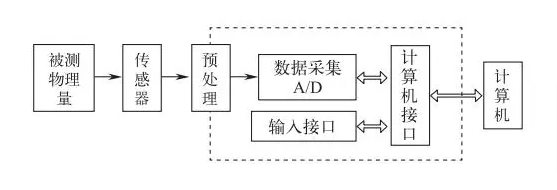
\includegraphics[angle=0,width=10cm]{./figure/2.1.png}
\caption{\label{2.1}智能传感器的基本结构}
\end{figure}

传感器负责设备信息检测和采集,计算机根据设定对输入信号进行处理,通过计算机接口与其他装置进行通信。智能传感器的实现可以采用模块式、集成式或混合式等结构。没有智能传感器,就不会有所谓的第四次工业革命,也就不会有智能城市应用,不会有智能交通,不会有智能制造。使用工业物联网技术,可以通过传感器实时感知数据,明确产品故障,生产过程中所有因素均能精确控制,才能真正实现生产智能化。掌握大数据,通过物联网和云计算的实际应用,才能实现企业的智能化高速发展。

\subsection{数据处理技术}
\label{sec:org26caa7d}
大数据与智能制造之间的关系可以总结为:制造系统中问题的发生和解决的过程中会产生大量数据,通过对这些数据的分析和挖掘可以了解问题产生的过程、造成的影响和解决的方式,这些信息被抽象化建模后转化成知识,再利用知识去认识、解决和避免问题,核心是从以往依靠人的经验(experience based),转向依靠挖掘数据中隐性的线索(evidence based),使得制造知识能够被更加高效和自发地产生、利用和传承。

工业大数据主要包含了各种工业产品与相关服务的所有数据,并在设计、制造、经营、服务等整个流程中形成,同时也包含工业互联网平台产生的各类数据。简单来说,工业大数据就是运用大数据、智能化等新技术、新手段解决工业发展面临的新需求、新问题,并创造新应用、新价值的过程\cite{林国军2023}。

根据企业的发展和管理以及大量客户和机构的研究与实践,我们可以提出工业大数据在企业运营管理过程中可落地的八大应用场景,如下图所示。

\begin{figure}[htbp]
\centering
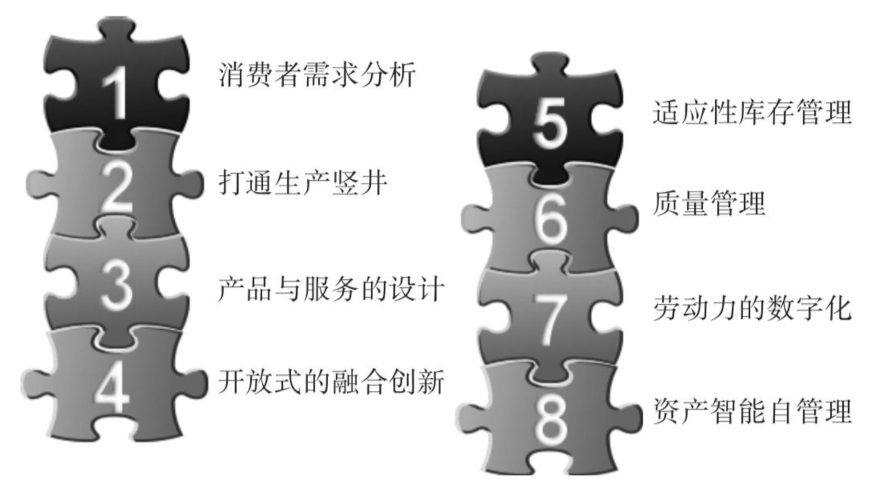
\includegraphics[angle=0,width=10cm]{./figure/2.2.png}
\caption{\label{2.2}工业大数据在企业运营管理中可落地的八大应用场景}
\end{figure}

按照美国国家标准与技术研究院(NIST)的定义,云计算是一种利用互联网实现随时随地、按需、便捷地访问共享资源池(如计算设施、存储设备、应用程序等)的计算模式。云计算可以按需提供弹性资源,它的表现形式是一系列服务的集合。结合当前云计算的应用与研究,其体系架构可分为核心服务、服务管理、用户访问接口3层。核心服务层将硬件基础设施、软件运行环境、应用程序抽象成服务,这些服务具有可靠性强、可用性高、规模可伸缩等特点,满足多样化的应用需求。服务管理层为核心服务提供支持,进一步确保核心服务的可靠性、可用性与安全性。用户访问接口层实现端到云的访问。

云计算的核心技术主要包括以下几个方面:虚拟化技术,是实现云计算资源池化和按需服务的基础;资源调度和管理技术,指在特定环境下,根据一定的资源使用规则,在不同资源使用者之间进行资源调整的过程;大规模数据处理技术,利用各种大数据模型,将一个任务分成许多子任务,使整个任务的完成时间有一定的保障;大规模信息通信技术,保证云计算服务的高可用性,但目前还处于发展阶段;大规模分布式存储技术,要求存储资源能够被抽象表不和统一管理,并以能够保证数据读写操作的安全性、可靠性、性能等各方面要求。

\subsection{智能控制技术}
\label{sec:orgbdfe0e5}
作为智能控制的基础,这里先对自动控制和机器视觉技术进行介绍。

自动控制原理是在不需人为操作和控制情况下,利用外置一些设备和装置,使某些大型机器设备按照系统参数自动规律运行\cite{黄慧媛2019}。自动控制原理已逐步形成了一套现代控制理论体系,随着计算机技术不断更新进步,依托于数学领域各项研究成果,自动控制理论正向着仿生学、人工智能为基础的智能控制方向不断发展\cite{蔡杰2018}。

机器视觉的发展主要经历了从黑白到彩色、从低分辨率到高分辨率、从静态到动态、从2D走向3D演变过程,其技术的迭代也是遵循相应的发展。机器视觉系统主要有照明电源、镜头、相机、图像采集/处理卡、图像处理系统、其他外部设备等组成,大体分为光学成像系统、图像捕捉系统、图像采集与数字化、智能图像处理与决策、控制执行器等,如图\ref{2.3}所示。

\begin{figure}[htbp]
\centering
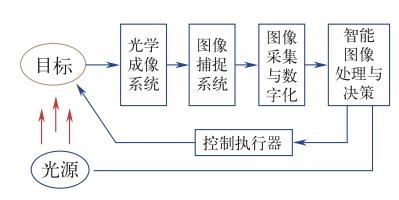
\includegraphics[angle=0,width=10cm]{./figure/2.3.jpg}
\caption{\label{2.3}机器视觉系统的基本结构}
\end{figure}

机器视觉技术在工业应用包括检验、计量、测量、定位、瑕疵检测和分拣,比如:汽车焊装生产线,检查四个车门和前后盖的内板边框所涂的反震和折边的胶条是否连续,是否有满足技术要求的高度;啤酒罐装生产线,检查啤酒瓶盖是否正确密封、装灌啤酒液位是否正确等质量检测,机器视觉参与的质量检验比人工检验要快准。在智能制造中,机器视觉技术常用于质量控制、精度测量、系统监控、安全监测、智能分拣等方面。

在控制论学派的观点中,感知、认知、反馈执行、迭代进化是实现智能的基本模式,其基本框架可以用图\ref{2.4}来表示。对某项任务的达成可以通过多个智能代理(Agent)的模式进行知识交互,通过事件和信息来驱动行动流程,利用微服务架构实现“信息—认知—知识—决策”的点对点思维逻辑,构建实体空间与赛博空间中个体空间、群体空间、环境空间、活动空间、推演空间的知识交互、知识共享、知识再生社区,从根本上解决信息系统知识生产速度无法满足知识消耗速度的矛盾,建立自主认知、自主成长的可持续发展的“知识创造”系统。

\begin{figure}[htbp]
\centering
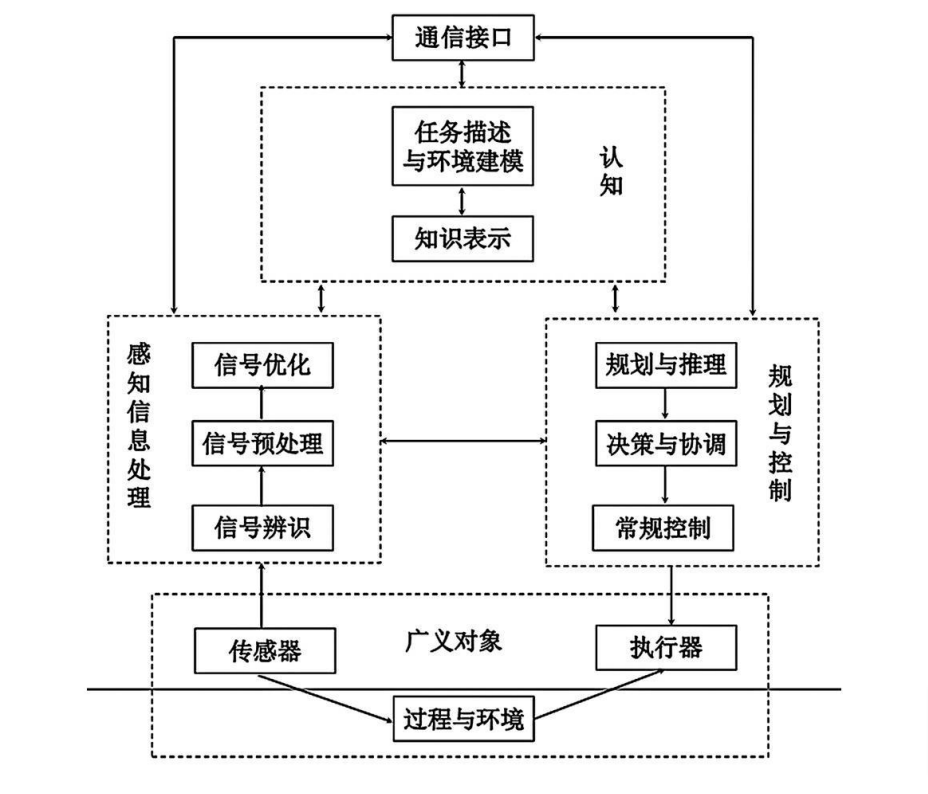
\includegraphics[angle=0,width=12cm]{./figure/2.4.png}
\caption{\label{2.4}智能控制系统的一般架构}
\end{figure}


智能控制是在自动控制的基础上,引入人工智能和机器学习技术,使控制系统具备自主学习和适应能力,能够根据不断变化的环境和任务,自动调整控制策略和参数,实现更高级别的控制性能。智能控制技术可以通过学习和优化算法,自动调整控制器的参数,适应系统的动态变化和非线性特性,提高控制系统的适应性和鲁棒性。

在实际应用中,自动控制、机器视觉和智能控制常常相互结合,共同应用于复杂的工程和系统中。例如,在制造业中,机器视觉可以用于产品质量检测和工艺控制,自动控制技术可以用于生产线的自动化控制,而智能控制技术可以结合机器视觉和自动控制,实现更智能化的生产过程和系统优化。

智能控制能克服传统控制理论的局限性,将控制理论方法和人工智能技术相结合,产生拟人的思维活动,采用智能控制的系统主要有以下特点:智能控制系统能有效利用拟人的控制策略和被控对象及环境信息,实现对复杂系统的有效全局控制,具有较强的容错能力和广泛的适应性;智能控制系统具有混合控制特点,既包括数学模型,也包含以知识表示的非数学广义模型,实现定性决策与定量控制相结合的多模态控制方式;智能控制系统具有自适应、自组织、自学习、自诊断和自修复功能,能从系统的功能和整体优化的角度来分析和综合系统,以实现预定的目标;控制器具有非线性和变结构的特点,能进行多目标优化。这些特点使智能控制相较于传统控制方法,更适用于解决含不确定性、模糊性、时变性、复杂性和不完全性的系统控制问题。

在智能控制系统的应用下,可以充分利用过往数据,与传统机电控制系统相比,在控制任务和控制目的方面更加复杂多样化,达到不断改善、升级、优化控制结构、控制体系的目的,进一步提升系统控制精准性、稳定性,有效提高生产率,进而不断推进企业工业化进程的发展\cite{邓玲黎2023}。

\subsection{人工智能技术}
\label{sec:org9306ba6}
在智能制造领域,人工智能(AI)技术扮演着重要的角色,其中机器学习和深度学习是最为常见和广泛应用的技术。

机器学习是一种人工智能技术,通过使用算法和模型,使计算机系统能够从数据中自动学习并改进性能,而无需明确的编程指令。在智能制造中,机器学习可以用于数据分析、模式识别、预测和优化等任务。通过对大量的生产数据进行学习和分析,机器学习可以发现隐藏在数据中的规律和模式,并帮助优化生产过程、改善产品质量和降低成本。

作为机器学习的一个分支,深度学习建立在人工神经网络的基础上,通过模拟人脑神经元之间的连接和信息传递,实现对复杂数据的学习和理解。深度学习在智能制造中被广泛应用于图像识别、语音识别、自然语言处理等任务。通过深度学习,计算机系统可以从大量的图像、语音或文本数据中提取特征,并进行高级的模式识别和理解,从而实现自动化的检测、分类和分析。

\begin{figure}[htbp]
\centering
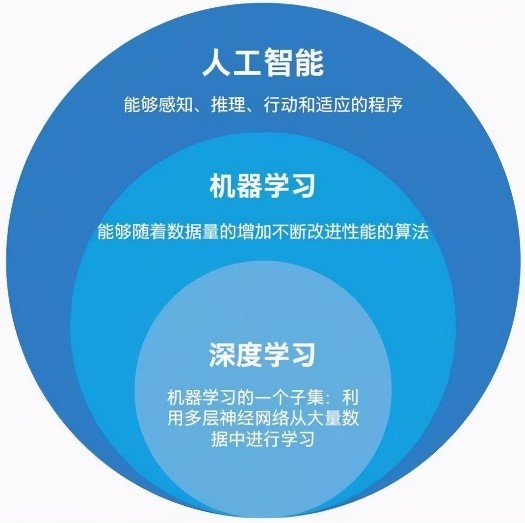
\includegraphics[angle=0,width=8cm]{./figure/2.5.jpg}
\caption{\label{2.5}人工智能、机器学习、深度学习的关系}
\end{figure}

通过机器学习和深度学习,智能制造系统可以根据数据和模式自动进行决策和优化,而不仅仅依赖人工经验和规则。智能制造中涉及大量的数据,包括生产数据、传感器数据、供应链数据等。机器学习和深度学习技术可以通过对这些数据的分析和挖掘,提供准确的预测能力,帮助优化生产计划、资源分配和供应链管理。通过预测需求、产品质量和设备故障等关键指标,智能制造系统可以实现更高效、灵活和可靠的生产。同时,机器学习和深度学习技术可以使智能制造系统具备自动化和智能化的能力。通过训练模型,系统可以学习和识别复杂的模式和规律,从而实现自主的决策和控制。例如,在自动化生产线上,机器学习和深度学习可以使机器人能够感知和适应环境,自动调整姿态和动作,实现高效的生产操作。

\subsection{智能加工技术}
\label{sec:orgea00db2}
智能加工是基于数字制造技术对产品进行建模仿真,对可能出现的加工情况和效果进行预测,加工时通过先进的仪器装备对加工过程进行实时监测控制,并综合考虑理论知识和人类经验,利用计算机技术模拟制造专家的分析、判断、推理、构思和决策等智能活动,优选加工参数,调整自身状态,从而提高生产系统的适应性,获得最优的加工性能和最佳的加工质效\cite{岳玮2015}。图\ref{2.6}为常见的智能加工流程。

\begin{figure}[htbp]
\centering
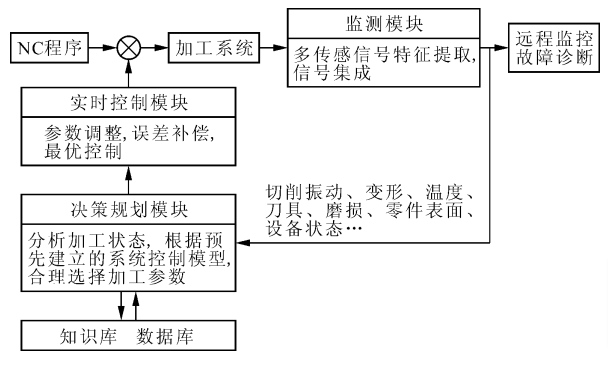
\includegraphics[angle=0,width=10cm]{./figure/2.6.png}
\caption{\label{2.6}智能加工实现流程}
\end{figure}

智能加工涉及到材料科学、信息科学、智能理论、机械加工学、机械动力学、自动控制理论和网络技术等多个学术领域。一般来说智能加工技术系统主要包括\cite{富宏亚2006}:建模仿真模块、过程检测模块、智能推理决策模块、最优过程控制模块。

数字孪生是客观事物在虚拟世界的镜像。创建数字孪生的过程,集成了人工智能、机器学习和传感器数据,以建立一个可以实时更新的、现场感极强的“真实”模型,用来支撑物理产品生命周期各项活动的决策。在完成对数字孪生对象的降价建模方面,可以把复杂性和非线性模型放到神经网络中,借助深度学习建立一个有限的目标,基于这个有限的目标,进行降价建模。利用数字孪生技术,对加工或者装配中的产品进行实时检测,可以提高产线的效率和良品率。

\begin{figure}[htbp]
\centering
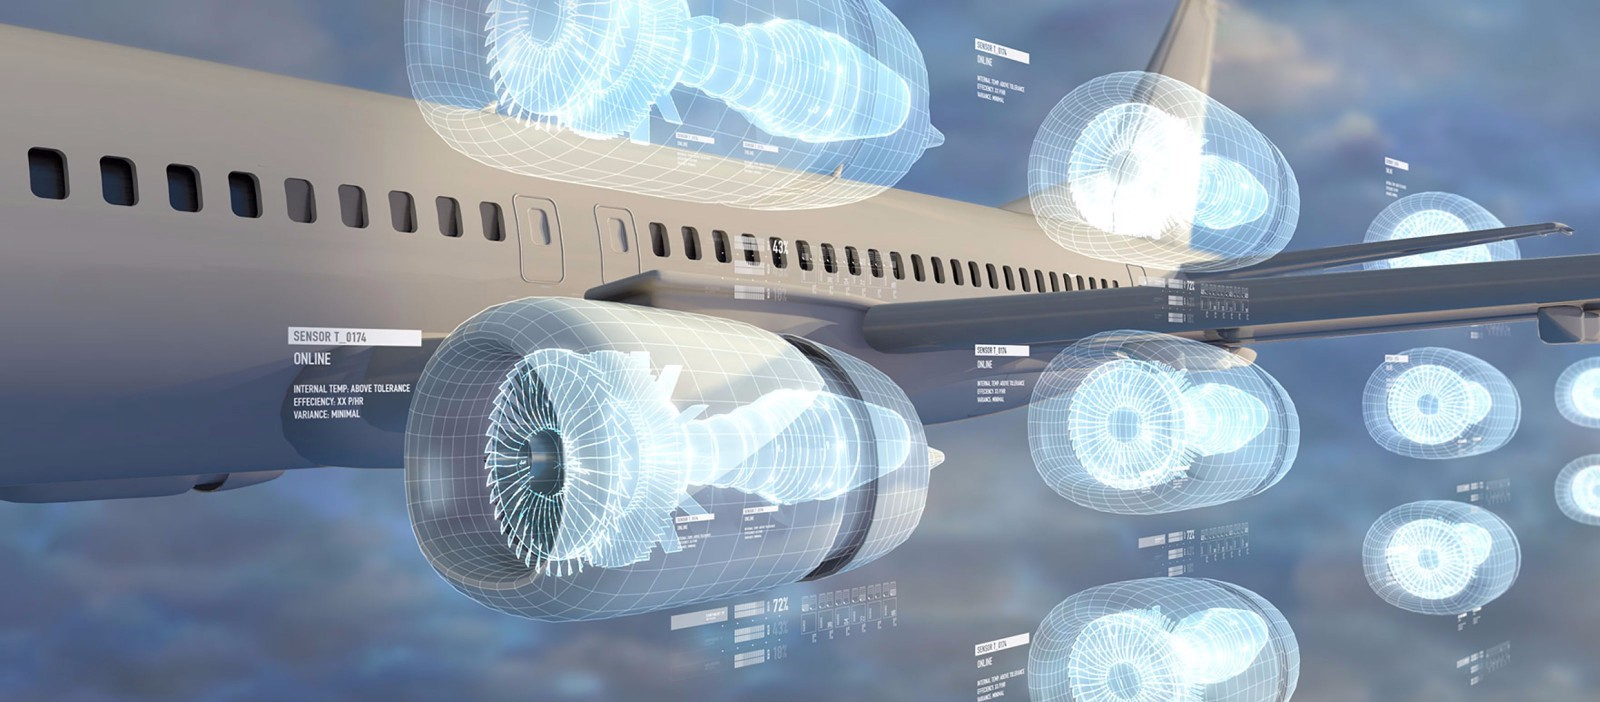
\includegraphics[angle=0,width=10cm]{./figure/2.7.jpg}
\caption{\label{2.7}飞机引擎的数字孪生}
\end{figure}

\subsection{工业机器人}
\label{sec:orgbdd8834}
在目前的工业领域中,制造机器人可以完全代替人进行重复、单调地生产作业,或者在危险、严酷的工作条件下进行加工。目前,国内外对工业机器人的定义大致分为两类\cite{王建兴2023}:

国际标准化组织(ISO)将其定义为:工业机器人是一种能够实现多种工作的可编程操作机,它具有自动控制以及多种操作的能力。

美国机器人学会定义(RIA)将其定义为:一种操作机器,它可以重复编程,并具有多种用途,在搬运、焊接等工序中被广泛使用;或一种特殊的系统,它具有可变化与可编程行为的操控装置,可完成不同类型的任务。

相对于传统人工,工业机器人存在以下优势\cite{周子又2023}:

生产效率高。工业机器人在制造领域中的应用,在提高工作效率的同时,也实现了人工劳动力的解放。以搬运机器人为例,只需要对搬运机器人进行相关参数设计,它就能完成高强度搬运工作,并且在长时间的工作中也不会感受到疲劳。既提高了搬运效率,也降低了人工劳动力负担,同时工业机器人在能源充足情况上能够实现持续性工作,在提高搬运效率的同时,也增加了作业安全性。

环境适应能力强。工业机器人经过特殊处理,能够适应于复杂的作业环境,更易完成较高难度、高危险性的工业生产。在危险性较高工作中,工业机器人的量化生产和修复能够充分降低危险源的影响程度,如在地质勘探、井底打捞等工作,只需要对工业机器人进行特定编码,就能完成相关工业作业,即使出现问题也符合工业生产承受范围内,极大地降低了制造生产中的安全事故发生。

生产精密度高。借助PLC编程技术、自动化技术、机器智能技术、液压驱动技术、智能控制技术等现代技术让工业机器人更适用于精密无尘的工业制造领域,编码程序的控制、机械功能模块化的操作让工业机器人操作更加精准、精细,能够高水平的完成相关工艺要求,相比于人工制造更易实现精密级的作用; 此外,工业机器人作业车间能够较好地完成无尘操作环境,大幅度降低人为因素和环境因素对工业制造产生的影响。

现阶段工业机器人在智能制造场景中已经有非常多的应用。主要在搬运、喷涂、焊接、加工和装配过程中使用。

在当前智能制造行业中,搬运机器人的市场份额较大,其次为装配式机器人,有关资料表明,搬运机器人在整个工业机器人市场中的占有率已达到 15\%以上。在实际的制造工序中,机器人技术可被运用到运输操作内部。在人工编程的帮助下,将搬运机器人引入现代工业。以此实现运输、存储以及包装等一系列自动化操作,既能使工人得到充分的解放,同时,有效地提升了运输工作的效率。

\begin{figure}[htbp]
\centering
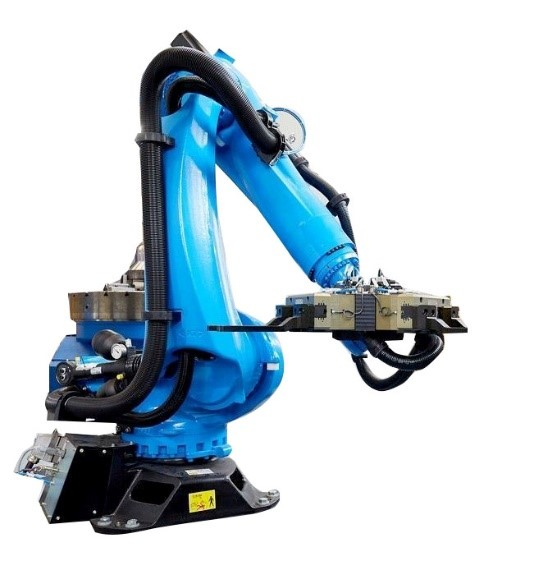
\includegraphics[angle=0,width=6cm]{./figure/2.8.jpg}
\caption{\label{2.8}搬运机器人}
\end{figure}

喷涂机器人的主要优点。柔性较大,应用领域广泛;改善喷淋品质,增加使用物料;使用方便,维修方便。可离线编程,可在现场进行大量的调试;装置效率较高,一般来说喷涂机器人工作效率可达到 90\%\textasciitilde{}95\%。喷涂机器人已被广泛地运用于各个领域,在智能制造领域内也已然展现出了全新的工业生产模式,经过这些年的发展,智能喷涂的产业雏形更为立体。

\begin{figure}[htbp]
\centering
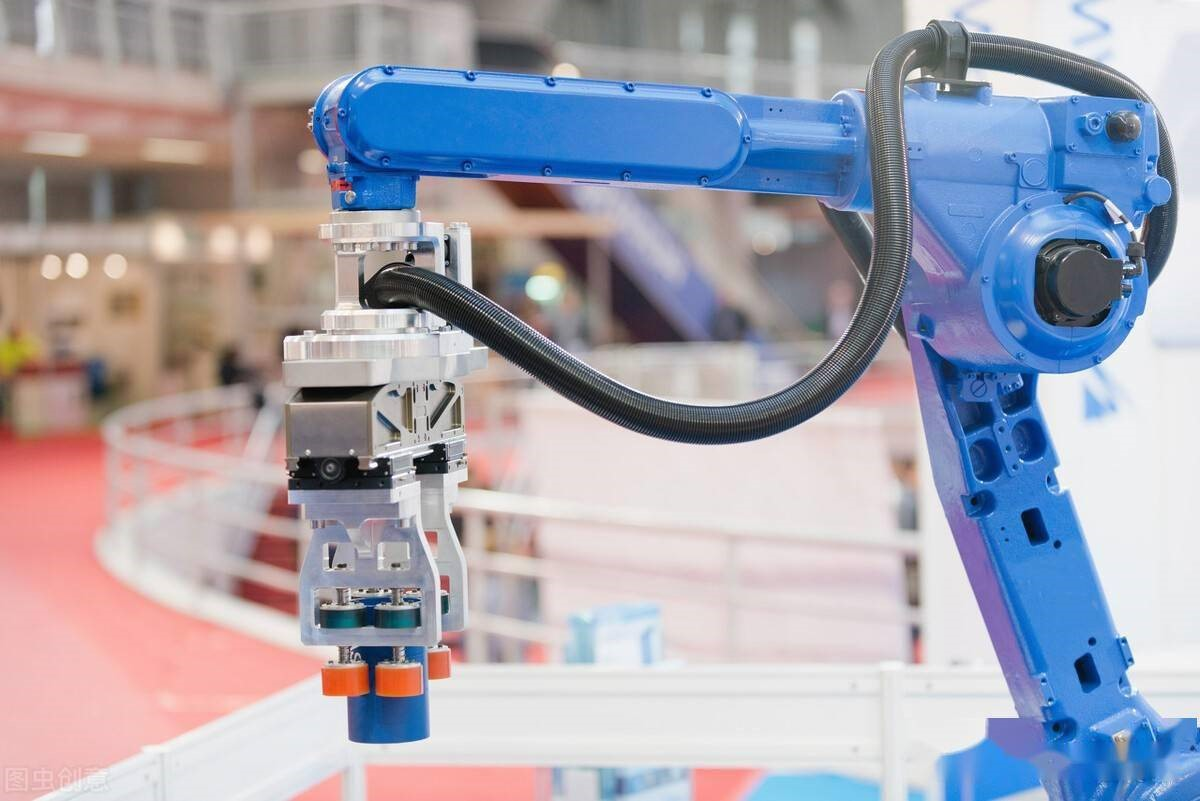
\includegraphics[angle=0,width=8cm]{./figure/2.9.jpg}
\caption{\label{2.9}生产线上的喷涂机器人}
\end{figure}

焊接机器人主要被运用于农机、船舶以及工程机械等领域内,现如今较为普遍,诸多领域由于对精密度要求较高,工作环境质量较差,因此,焊接工作具有很大的劳动强度。

\begin{figure}[htbp]
\centering
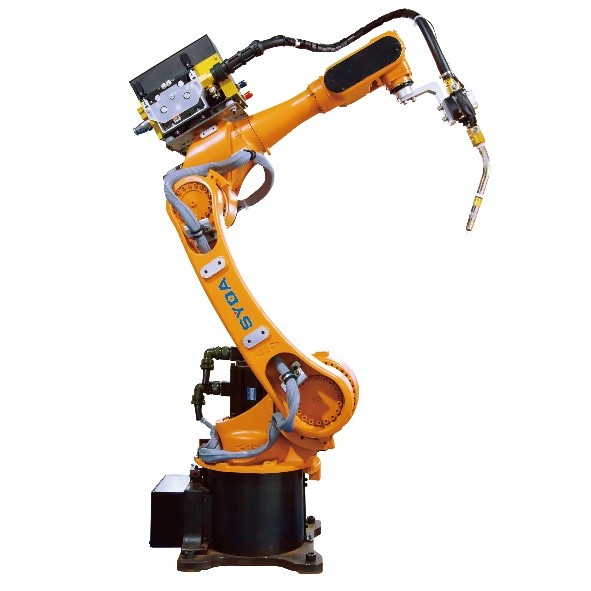
\includegraphics[angle=0,width=6cm]{./figure/2.10.jpg}
\caption{\label{2.10}焊接机器人}
\end{figure}

随着制造业不断向智能化、信息化的方向发展,工业机器人在机械加工等过程中运用较为广泛,其中包括打磨、抛光、钻削、铣削、钻孔等。在工业生产中,装配机器人已是一种比较普遍的产品。装配机器人属于工业机器人,其目的是实现组装作业。组装机器人由操作机、控制器以及末端执行器等构件组成,也属于FMS 中的关键部件。

工业机器人的发展实现了传统制造业的有效变革,特别是基于人工智能技术、虚拟仿真技术赋能下工业机器人应用场景更加多元化,作业范围更加广泛。随着技术的进步和创新,工业机器人的功能和应用领域不断扩展,将为未来的智能制造提供更多可能性。

\subsection{工业互联网平台}
\label{sec:org7d30be9}
20世纪70年代中期,美国Xerox公司提出了“以太网”这个新概念,首次提出采用一种传输媒介将Xerox打印机与数个计算机相连进行通信的构思,即带冲突检测的载波侦听多路访问(CSMA/CD)的方法。40多年以来,随着科技的不断发展,这一设想在实践中得到了不断的改进,从而形成一致而又强大的局域网技术。IT工程师从实际应用出发采取各种措施改进以太网技术,今天,作为物理层基础的以太网与最广泛的、标准化的通信协议TCP/IP有机结合,成为现代通信技术最成熟的使用方法。

工业互联网是办公领域以太网技术在控制网络延伸的产物。由于与办公以太网网络的应用对象不同、使用环境不同、数据通信量和实时性不同,工业互联网产生了各种特定的要求。在工业应用场合中,构成一个通信网络的组成部分是非常复杂的。除了需要计算机外,更主要的是必须与各种不同类型的控制器(如PLC、CNC、IPC)、不同类型的变送器(如压力、温度、液位、红外线、位移等变送器)、不同类型的执行器(如变频器、直流调节系统、机器人控制系统)、现场总线I/O系统、人机界面等连接,同时连接于因特网,通过Web技术进行远程监控等。构成工业互联网的通信技术必须更快速,传输的确定性更高。为了解决在不间断的工业应用领域,在极端条件下网络也能稳定工作的问题,工控厂家专门开发和生产了导轨式集线器、交换机产品并安装在标准DIN导轨上,且有冗余电源供电,接插件采用牢固的DB-9结构。而在IEEE 802.3af标准中,对以太网的总线供电规范也进行了定义。此外,在实际应用中,主干网可采用光缆传输,现场设备的连接则可采用屏蔽双绞线,对重要的网段还可采用冗余网络技术,以提高网络的抗干扰能力和可靠性。为了解决实时性问题,产生了PROFINET、Modbus TCP、EtherCAT等多种实时工业以太网协议。

工业互联网层次结构可以分为3层,包含基础设施层(IaaS)、平台层(PaaS)、应用层(SaaS)三大层级,具体如图\ref{2.11}。

\begin{figure}[htbp]
\centering
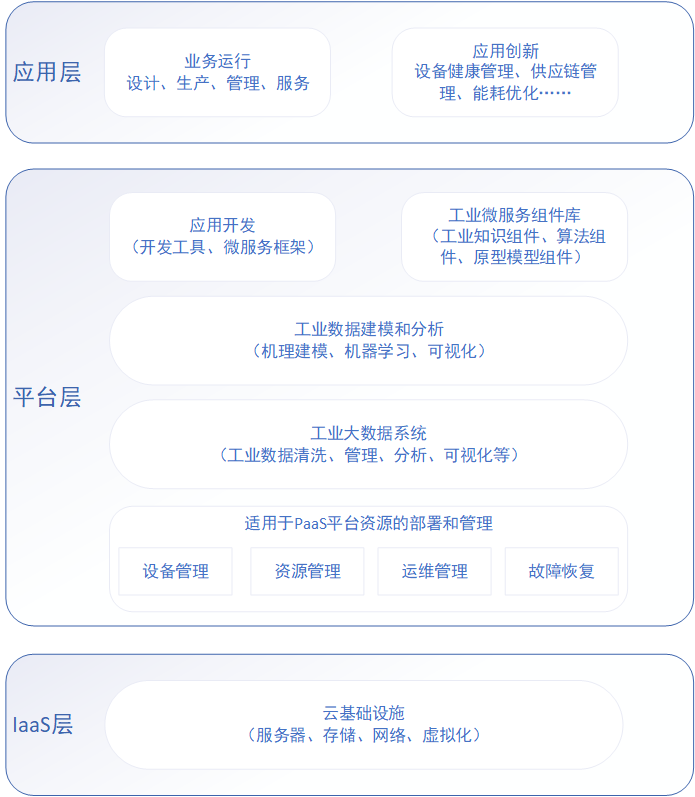
\includegraphics[angle=0,width=10cm]{./figure/2.11.png}
\caption{\label{2.11}工业互联网的层次结构}
\end{figure}

基础设施层是工业互联网平台的运行基础,由IT基础设施提供商为平台建设与运营提供虚拟化的计算资源、网络资源、存储资源,为平台层、应用层的功能运行、能力构建及服务供给提供高性能的计算、存储、网络等云基础设施。

平台层是工业互联网平台的核心,由平台建设运营主体、各类微服务组件提供商、边缘解决方案提供商等共同建设,提供应用全生命周期服务环境与工具、IT微服务库、工业大数据管理等功能,依托强大的大数据处理能力、开放的开发环境工具,向下接入社会开放资源,向上支撑工业APP的开发部署与运行优化,发挥着类似于“操作系统”的重要作用。

应用层是工业互联网平台的关键,通过激发全社会力量,依托各类开发者基于平台提供的环境工具、资源与能力,围绕特定应用场景形成一系列工业APP,通过实现业务模型、技术、数据等软件化、模块化、平台化,加速工业知识复用和创新。各类工业APP的大规模应用将有效促进社会资源的优化配置,加快构建基于平台的开放创新生态。


工业互联网平台是工业互联网在智能制造中应用的具体形式\cite{李亚敏2023}。工业互联网平台的基础是数据采集,一方面,随着加工过程和生产线精益化、智能化水平的提高,必须从多角度、多维度、多层级来感知生产要素信息。另一方面,工业互联网平台也需要进行高效的海量、高维、多源异构数据融合,进一步实现跨部门、跨层级、跨地域生产要素之间的关联和互通。工业互联网平台的核心是平台。工业互联网平台在通用PaaS架构上进行二次开发,实现工业PaaS层的构建,为工业用户提供海量工业数据的管理和分析服务,并能够积累沉淀不同行业。工业互联网平台的关键是应用。一方面,工业互联网平台的使用对象是人,其最终推送的决策,必须是人可以直观接收和理解的;另一方面,对于用户不同的要求,工业互联网平台需要基于新模式的生产场景和个性化的生产需求,利用数据分析方法,推送定制化的决策方案。

\section{智能制造的应用场景}
\label{sec:org125382e}
\subsection{智能制造系统}
\label{sec:orgeee4a75}
智能制造系统是基于信息技术和智能化技术,将传统的制造过程与先进的数字技术、自动化技术和人工智能相结合,实现生产过程的数字化、网络化和智能化。它涵盖了从产品设计到生产制造、供应链管理和服务的全过程。

智能制造系统的主要组成部分包括以下方面:

数字化设计和仿真:智能制造系统中的产品设计和开发阶段采用数字化的方法进行,包括计算机辅助设计(CAD)、计算机辅助工程(CAE)和计算机辅助制造(CAM)。通过虚拟仿真和模拟技术,可以在实际制造之前对产品进行测试和优化,提高产品质量和减少开发时间。

智能生产和自动化:智能制造系统实现了生产过程的智能化和自动化。它包括生产设备的自动控制、生产线的自动化运行、物料搬运的自动化和机器人的应用。通过采用先进的传感器、执行器和控制系统,实现生产过程的高效、灵活和精确控制,提高生产效率和质量。

数据集成和共享:智能制造系统通过物联网、云计算和大数据技术,实现生产过程中数据的采集、存储和分析。它可以将来自各个环节的数据整合在一起,形成全面的生产数据,为决策提供支持。同时,还可以实现数据的共享和协同,提高生产过程中各个环节的协调性和响应能力。

智能决策和优化:智能制造系统利用数据分析、机器学习和人工智能技术,对生产数据进行挖掘和分析,从中提取有价值的信息和知识,支持实时决策和优化。通过实时监测和分析生产过程中的数据,可以预测问题和故障,调整生产计划,优化资源配置,提高生产效率和灵活性。

一般的智能制造系统结构如下图。
\begin{figure}[htbp]
\centering
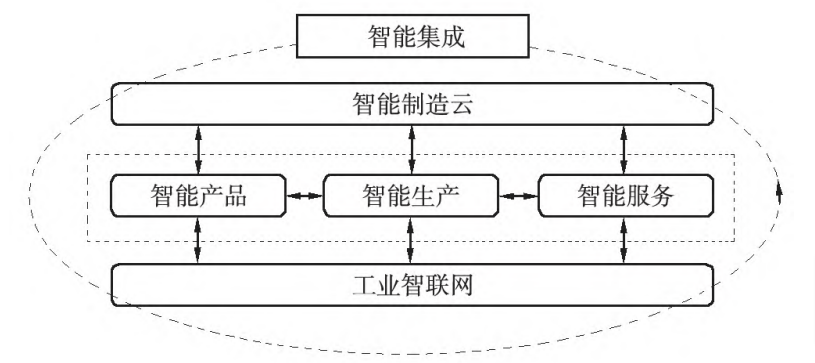
\includegraphics[angle=0,width=10cm]{./figure/3.1.png}
\caption{\label{3.1}现代智能制造系统架构}
\end{figure}

企业主要面临工艺优化、智能控制、生产调度、物料平衡、设备运维、质量检验、能源管理和安全环保等核心问题,通过基础数字化、网络化互联和智能化应用路径实施,基于企业短期需求、中期和长期规划,还要考虑行业的自动化、信息化和数字化等技术基础条件基础上进行智能制造顶层设计,使智能制造系统架构不仅具备重构行业整体价值链、重构业务流程和商业模式,而且还应具有面向未来持续迭代创新能力\cite{柴春蕾2021}。该智能制造系统架构包括智能产品、智能生产、智能服务、工业智联网和智能云。


\subsection{智能制造装备}
\label{sec:org35308ca}
智能制造装备是一种由智能机器和人类专家共同组成的人机一体化智能系统,它在制造过程中能进行智能活动,如分析、推理、判断、构思和决策等\cite{傅建中2014}。通过人与智能机器的合作共事,去扩大、延伸和部分地取代人类专家在制造过程中的脑力劳动。智能制造装备最终要从以人为主要决策核心的人机和谐系统向以机器为主体的自主运行方向转变。

智能制造装备是智能制造体系中的重要组成部分,包括工业机器人、自动化生产线、智能仓储物流系统、数字化车间等。

工业机器人是智能制造装备中的重要组成部分,主要用于生产线上的自动化生产。它们可以执行各种任务,例如搬运、装配、切割、焊接和喷涂等,可以提高生产效率、降低生产成本、保障生产质量。自动化生产线是指利用自动化技术实现的生产线,可以在生产过程中自动完成各个工序的加工,提高生产效率,降低生产成本,同时提高生产质量。智能仓储物流系统是利用物联网、RFID等技术,实现智能化的仓储物流系统,可以实现自动化的仓储、管理、运输等功能,提高物流效率和管理水平。数字化车间是指通过工业互联网技术、物联网技术等手段实现生产线数字化、智能化的车间。数字化车间可以对生产数据的实时监控和分析,实现生产过程的优化和智能化管理。

根据工业和信息化部制定和发布的《智能制造装备产业“十二五”发展路线图》规划\cite{工业和信息化部2012},智能制造装备的发展重点为:

(1)九大关键智能基础共性技术,包括:①新型传感技术;②模块化、嵌人式控制系统设计;③先进控制与优化技术;④系统协同技术;⑤故障诊断与健康维护技术;⑥高可靠实时通信网络技术;⑦功能安全技术;⑧特种工艺与精密制造技术;⑨识别技术。

(2)八项核心智能测控装置与部件,包括:①新型传感器及其系统;②智能控制系统现场总线;③智能仪表;④精密仪器;⑤工业机器人与专用机器人;⑥精密传动装置;⑦伺服控制机构;⑧液气密元件及系统。

(3)八类重大智能制造成套装备,包括:①石油石化智能成套设备集成;②冶金智能成套设备集成;③智能化成形和加工成套设备集成;④自动化物流成套设备集成;⑤建材制造成套设备集成;⑥智能化食品制造生产线集成;⑦智能化纺织成套装备集成;⑧智能化印刷装备集成。

(4)六大重点应用示范推广领域、包括;①电力领域;②节能环保领域;③农业装备领域;④资源开采领域;⑤国防军工领域;⑥基础设施建设领域。


智能制造装备是高端装备的核心,是制造装备的前沿和制造业的基础,已成为当今工业先进国家的竞争目标。作为高端装备制造业重点发展方向和信息化与工业化深度融合的重要体现,发展智能制造装备产业对于加快制造业转型升级,提升生产效率、技术水平和产品质量,降低能源资源消耗,实现制造过程的智能化和绿色化发展具有重要意义[12]。

\subsection{智能产品服务}
\label{sec:orga93e423}
一般的经济学领域认为服务具有典型的无形性、不可分离性和不可存储性三个单行特征,在对智能产品服务生态系统进行详细剖析之后,将其服务的特征拓展为八个子项,包含了增值性、流程性、集成性、可持续性、无形性、不可分离性、差异性和不可存储性八个子项\cite{郑茂宽2018}。

智能产品服务包括以用户为中心的产品全生命周期的各种服务,服务智能化将大大促进个性化定制等生产方式的发展,延伸发展服务型制造业和生产型服务业,促进生产模式和产业形态的深度变革。通过持续改进,建立高效、安全的智能服务系统,实现服务和产品的实时、有效、智能化互动,为企业创造新价值。智能服务关键技术包括:云服务平台技术、预测性维护技术、个性化生产技术以及增值服务技术。

云服务平台技术是实现智能服务的重要保障,是实现用户与制造商信息交互的核心技术。云服务平台具有多通道的并行接入能力,可以通过传感器等对产品的制造过程,装备的运行状态,用户的使用习惯、需求信息等数据进行采集和处理。一方面,通过用户需求分析,引导制造商生产满足用户需求的个性化产品;另一方面,通过对装备运行状态、用户使用习惯进行分析,从而为用户提供有效的增值服务,进而提升产品附加值和企业收益。

预测性维护是以产品状态为依据而提供的维护或者保养建议,从而避免产品失效而造成的不良后果,同时还可以有效提升产品附加价值。传统的预测性维护针对的是制造中的生产设备而言,但是广义的预测性维护针对的是产品相关的全部生产因素。在产品使用过程中,针对主要部位进行定期(或连续)的状态监测,从而确认产品所处的运行状态。预测性维护是智能制造未来的发展趋势,依据产品的状态发展趋势和可能的故障模式,制定预测性维修计划,确定产品应该维修的时间、内容、方式和必需的技术和物资支持等。预测性维修集状态监测、故障诊断、故障(状态)预测、维修决策支持和维修活动于一体,是一种新兴的维护方式。

个性化生产服务,是智能制造的未来发展方向之一。通过将个性化的服务融入产品,提升产品附加值,可以为企业创造新的价值。个性化生产服务通过云服务平台收集客户个性化需求,按照顾客需求进行生产,以满足顾客的个性化需求。由于消费者的个性化需求差异性大,加上消费者的需求量又少,因此企业实行定制生产必须在管理、供应、生产和配送各个环节上,都必须适应这种多品种、小批量、多式样和多规格产品的生产和销售变化。

增值服务技术,主要体现在产品销售后,以服务应用软件为创新载体,通过大数据分析、人工智能等新兴技术,结合最新的5G通信手段,自动生成产品运行与应用状态报告,并推送至用户端,从而为用户提供在线监测、故障预测与诊断、健康状态评估等增值服务。与此同时,利用云服务平台,收集用户在产品使用过程中的行为信息等数据,针对不同客户的习惯,提供个性化的升级服务,从而有效地增加产品附加值,为企业创造新的价值。

\subsection{智能制造工厂}
\label{sec:org8b3b9d7}
从宏观理论上讲,智能工厂是智能化技术运用到一定时期的产物,它主要是利用现有计算机网络技术和信息自动化设备来提升制造业的整体水平和企业经济效益。现阶段,我国现有的智能工厂主要包含:物理设备、管理系统以及庞大的信息数据库等多个领域的信息与技术\cite{杨鹏2019}。

智能工厂是未来工厂的发展趋势,顾名思义,智能工厂最大的特性就是智能。智能工厂既是一个由机器、通信机制和计算能力构成的互联网络,也是一个信息物理系统,该系统能够利用人工智能 (AI) 和机器学习等先进技术分析数据、驱动自动化流程并不断学习。在未来工厂中,基础劳动力将会被机器所取代,黑灯工厂、无人工厂将会成为智能制造型工厂发展的主流趋势。

\begin{figure}[htbp]
\centering
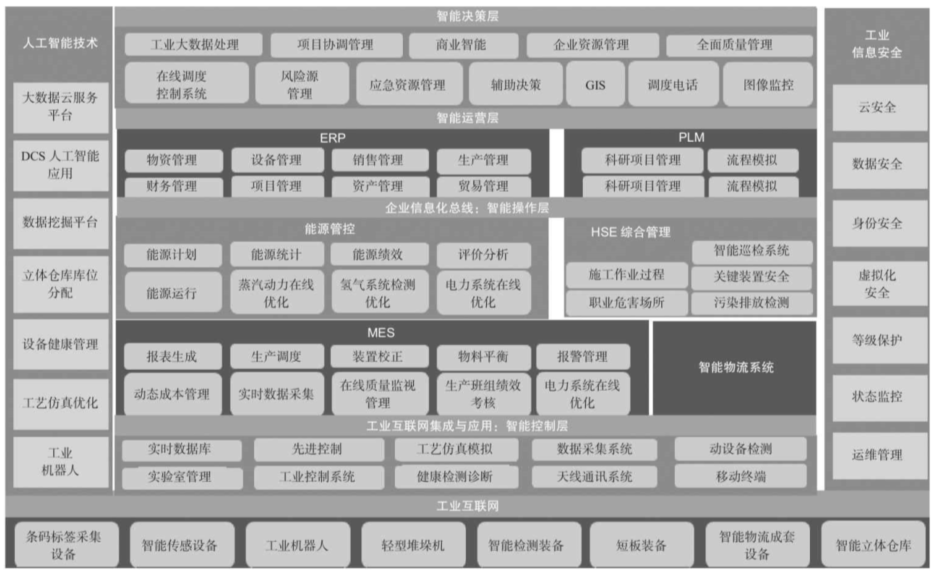
\includegraphics[angle=0,width=10cm]{./figure/3.2.png}
\caption{\label{3.2}智能工厂的整体构架示例}
\end{figure}

数字化智能工厂将机器、人员和大数据整合到统一的数字互联生态体系中。数字化智能工厂不仅能够管理和分析数据,还能从经验中学习。此外,智能工厂还能解读数据集并从中获取洞察,进而预测趋势和事件,并推荐和实施智能制造工作流和自动化流程。智能工厂可以通过持续优化相关程序,实现自我校正和优化。也就是说,智能工厂能够自己学习并为人类提供指导,从而增强韧性,提高生产力和安全性。

工业4.0智能工厂的结构大致分为三步:

数据采集:在工业4.0智能工厂中,利用人工智能和现代数据库技术,管理和获取分散在企业内部、供应链和世界各地的有用数据集。通过利用各种传感器和网关,工业物联网 (IIoT) 支持互联的机器将数据收集到系统中。借由各种其他数据门户,人工智能系统可以整合与绩效、市场趋势、物流或任何其他潜在相关来源有关的数据集。

数据分析:机器学习和智能业务系统使用高级分析和现代数据管理解决方案来充分利用收集的所有数据。工业物联网传感器可以在机器需要维修或维护时发出警报。这些系统不仅可以整合市场和运营数据,帮助企业发现机遇和风险,还能持续研究工作流的效率,从而优化绩效,并实施必要的自动校正。事实上,通过比较和分析数据集,系统可以构建无限的组合,为数字工厂优化和供应链预测提供有力支持。

智能工厂自动化:工业4.0智能工厂的一大优势在于它能够创建自动化的工作流程,一旦数据采集和分析工作完成,系统就会建立起相关的工作流,并将工作说明下发给系统中的机器和设备。这些设备可能位于工厂内部,也可能位于供应链中的物流或制造环节。智能工厂会不断地监控并优化智能工作流和流程。如果新闻报道提醒某产品的需求将激增,系统就可以指示 3D 打印机工作流提高该产品的生产优先级。如果原材料装运延迟,则可以利用库存缓冲来避免任何形式的供应中断。

\section{智能制造前沿趋势}
\label{sec:orgfbc659a}
\subsection{智能制造的国际发展}
\label{sec:org6cf3059}
自20世纪80年代末智能制造的概念出现后,为了在开创和全面推进高技术战略智能化工业的时代进程中发挥主导力量,以欧(德)、美、日为主的发达工业国家纷纷将智能制造列入国家级计划并着力发展。其中,美国着眼于未来的军事需求,对武器装备的智能制造格外重视;欧盟在航宇和防务的智能化制造领域也持续开展跨国合作。
\begin{enumerate}
\item 德国工业4.0
\label{sec:orgd74d5ae}

\setlength{\parindent}{2em}
德国凭借强大的机械和装备制造业、占据全球显著地位的信息技术能力,以及在嵌入式系统和自动化工程领域具有的高技术水平,在工业制造方面一直处于欧洲领头羊的地位,是全球制造业中最具竞争力的国家之一。为了应对来自美国、日本和中国在未来工业制造上的竞争,德国一直在寻求战略方案,并且提出了“智能工厂”、“工业4.0”等构想,希望在所谓第四次工业革命的道路上起到引领作用。

“工业4.0”计划是德国2012年3月正式启动的“高技术2020战略行动计划”列出的十大“未来计划”之一,参与者包括代表德国教育与研究部的德国国家科学与工程院、德国人工智能研究中心、弗劳恩霍夫研究所、“‘东威斯特法伦-利普’智能技术系统”尖端研究组、“智能工厂”计划,以及西门子、博世、FESTO、TRUMPF、SAP等德国领先的工业和软件企业\cite{Bunse2013}。

目前,德国建立了“工业4.0平台”,由德国信息技术/通讯和新媒体协会(BITKOM)、德国机械设备制造业联合会(VDMA)以及德国电气和电子工业联合会(ZVEI)3个专业协会共同建立秘书处,为关键的优先主题制订研发路线图。这3个协会在2013年初进行了“工业4.0前景”调查,对278家企业的调查显示,47\%的企业已经积极参与“工业4.0”计划,18\%的企业参加了对该计划的研究,12\%的企业则已经开始实施“工业4.0”计划。

“工业4.0”计划已经从德国“高技术2020战略行动计划”处获得2亿欧元投资,启动了包括信息物理生产系统、信息通信技术2020、工业4.0自动化等至少45个研究项目,2012年启动的“‘东威斯特法伦-利普’智能技术系统”尖端研究组是其中最大的项目。此外,在“高技术2020战略”框架下开展的“信息通信技术(ICT)2020——创新研究”计划以及“智能服务——基于网络的商业服务”计划都与“工业4.0”密切相关。

德国“工业4.0”计划的要点可以概括为:建设一个网络、研究三大主题、实现三项集成、实施八项计划。软件密集型嵌入式系统是德国的强项,在“工业4.0”中继续作为发展的一个核心,信息物理系统就衍生自网络化嵌入式系统,并将最终前进到物联网、数据和服务互联网,这也是“工业4.0”的一个愿景。能够表现“工业4.0”的中心特征的3个范本是智能产品、智能机床和增强的操作员。

\begin{figure}[htbp]
\centering
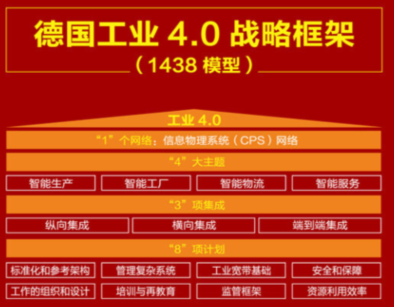
\includegraphics[angle=0,width=10cm]{./figure/4.1.png}
\caption{\label{4.1}德国工业4.0战略框架(1438模型)}
\end{figure}

总的来看,“工业4.0”计划的核心就是通过信息物理系统网络实现人、设备与产品的实时连通、相互识别和有效交流,从而构建一个高度灵活的个性化、数字化的智能制造模式。在这种模式下,生产由集中向分散转变,规模效应不再是工业生产的关键因素;产品由趋同向个性转变,未来产品都将完全按照个人意愿进行生产,极端情况下将成为自动化、个性化单件制造;用户由部分参与向全程参与转变,用户不仅出现在生产流程的两端,而且广泛、实时参与生产和价值创造的全过程。

德国学术界和工业界将制造业领域的技术渐进性进步描述为工业革命的四个阶段,即“工业4.0”的进化历程。在未来,基于信息物理系统的智能化将使人类步入以智能制造为主导的第四次工业革命。产品全生命周期和全制造流程的数字化以及基于信息通信技术的模块化集成,将形成一个高度柔性、定制化、数字化的产品与服务的生产模式,即实现“工业4.0”。

\item 美国制造业再兴计划
\label{sec:org97709ac}

美国的制造业总产值从1895年取代大英帝国成为世界第一之后,一直到2009年被中国取代。目前,中美两国的制造业总产值非常接近。事实上,如果单列,美国的制造业将是世界上的第9大经济体。美国的制造业占美国总研发经费的70\%,出口额的69\%,专利的90\%。在制造业中每生产1美元的产品会在其他服务活动中,像工程设计、物流管理、运输和销售,产生1.37美元的价值。在制造业部门,每小时报酬平均超过32美元,约比服务行业高出22\%。然而制造业就业人数占总就业人数的百分比自1950年一直在下降,制造业就业的总人数及制造业的就业机会自1979年以来一直在减少。与之相反的是服务业,在1950,美国家庭67\%的消费支出花在了消费类产品上,33\%在服务上。到2008年,美国家庭42\%的消费支出花在了消费类产品上,58\%在服务上。随着收入增加,消费者对服务的需求(如旅游、外出就餐和医疗机构)增速往往会快于对消费类产品的需求,如汽车和电子产品。

近年来,为了重塑美国制造业的全球竞争优势,美国启动了制造业振兴战略\cite{张婉姝2018},加快发展技术密集型先进制造业,实现再工业化。作为先进制造业的重要组成部分,智能制造得到了美国政府、企业各层面的高度重视。美国政府启动了一系列计划和项目以对基于模型的企业、信息物理系统、工业机器人、先进测量与分析、智能制造系统集成等智能制造关键要素的发展进行系统支持。

作为率先提出智能制造的国家,美国于1992年开始执行新技术政策,大力支持所谓的“关键重大技术”,包括信息技术和新的制造工艺,而智能制造技术也列入其中。在1995年启动的国际“智能制造系统”(IMS)十年期研究计划中,美国有122家企业和组织积极参与,目前仍旧同欧盟等一起作为IMS计划的核心成员。美国能源部、商务部国家标准与技术研究院(NIST)和国家科学基金(NSF)是智能制造的重要支持力量,近年来资助并设立了众多研究项目,推动其发展,这其中就包括美国“智能制造领导力联盟”计划。2006年,NSF提出了信息物理系统的概念,并与NIST一起给予大力支持。2014年12月,美国政府宣布,国家制造创新网络中“智能制造创新机构”的组建工作将由能源部牵头启动,该机构将开发并推广包括先进传感器和复杂工艺控制在内的智能制造新技术。

美国国防部一直是智能制造的积极推动者,先后启动了一系列计划和项目,以对武器装备研制生产中的智能制造进行研究与实践。在2005年启动的“下一代制造技术计划”中,国防部确定了6个重点领域,其中就包括基于模型的企业、智能系统、企业级集成、知识应用等面向智能制造的领域。2010年,国防部制造技术计划增加了“先进制造企业”投资科目,汇集了全数字化打通、制造网络连接、智能制造规划与执行等有关智能制造领域的研究方向。国防预先研究计划局(DARPA)于2010年启动的“自适应运载器制造”(AVM)项目使大型复杂系统制造在设计和制造的部分环节实现了智能化。国防部2014年牵头成立的“数字化制造和设计创新机构”的使命之一就是在智能制造方面引领创新,并将与AVM项目相结合,将研究成果转化到武器装备研制生产中。

此外,GE公司作为世界最大的多元工业集团,也提出了自己的“工业互联网”概念。与工业4.0的基本理念相似,它同样倡导将人、数据和机器连接起来,形成开放而全球化的工业网络,但其内涵已经超越制造过程以及制造业本身,跨越产品生命周期的整个价值链,涵盖航空、能源、交通、医疗等更多工业领域。GE公司预测,如果工业互联网能够使生产率每年提高1\%\textasciitilde{}1.5\%,那么未来20年,它将使美国人的平均收入比当前提高25\%\textasciitilde{}40\%。如果世界上其他地区能确保实现美国生产率增长的一半,那么工业互联网在此期间会为全球GDP增加10\textasciitilde{}15万亿美元。

\item 中国制造2025
\label{sec:org7e62434}

新一轮科技革命和产业变革,正在带来国际产业分工格局的重塑与洗牌,而与中国加快产业结构调整的历史性交汇,也迫使中国必须实施创新驱动发展战略。

2015年5月19日,李克强总理签批了《中国制造2025》,部署全面推进实施制造强国战略。这是我国实施制造强国战略第一个十年的行动纲领。德国工业4.0跟中国制造2025的区别是,德国是提出信息物理系统,积极布局智能工厂、推进智能生产;中国是大力发展智能制造和信息制造模式。两个战略的共同点都是为了迎接新一轮科技和产业革命的到来,着眼于以数字化和网络化为主的智能化生产,不同点是:两国制造基础不一样,德国是制造业强国,中国是制造业大国,中国制造占世界制造市场的20\%,但是有点儿虚胖;两国制造业的发展阶段不一样,德国已经完成了工业3.0,中国尚处在工业2.0,部分达到工业3.0,所以德国是从工业3.0串联到工业4.0,中国是从工业2.0、工业3.0一起并联到工业4.0\cite{高潮2016}。中国的产业形态分布不均,既有很先进的现代化工厂,也有前店后厂的夫妻店工厂,发展极不均衡,但是未来十年是中国制造业走向智能化的十年,如果不能走向智能化将会被市场所淘汰。

2015年7月16-18日,习近平主席在吉林长春考察了两家装备制造企业。他强调要把装备制造业作为重要产业,加大投入和研发力度,奋力抢占世界制高点、掌控技术话语权,使我国成为现代装备制造大国和强国。2015年7月9日和10日,李克强总理连续主持召开两场座谈会,多次强调实施“中国制造2025”行动,加快促进新动力转换。两位最高领导人同时为制造业鼓劲,凸显了制造业在国民经济中突出的重要地位。

“中国制造2025”是升级版的中国制造,体现为4大转变、1条主线和8项战略对策。4大转变:一是由要素驱动向创新驱动转变;二是由低成本竞争优势向质量效益竞争优势转变;三是由资源消耗大、污染物排放多的粗放制造向绿色制造转变;四是由生产型制造向服务型制造转变。1条主线,是以体现信息技术与制造技术深度融合的数字化、网络化、智能化制造为主线。8项战略对策:推行数字化、网络化、智能化制造,提升产品设计能力,完善制造业技术创新体系,强化制造基础,提升产品质量,推行绿色制造,培养具有全球竞争力的企业群体和优势产业,发展现代制造服务业。

\begin{figure}[htbp]
\centering
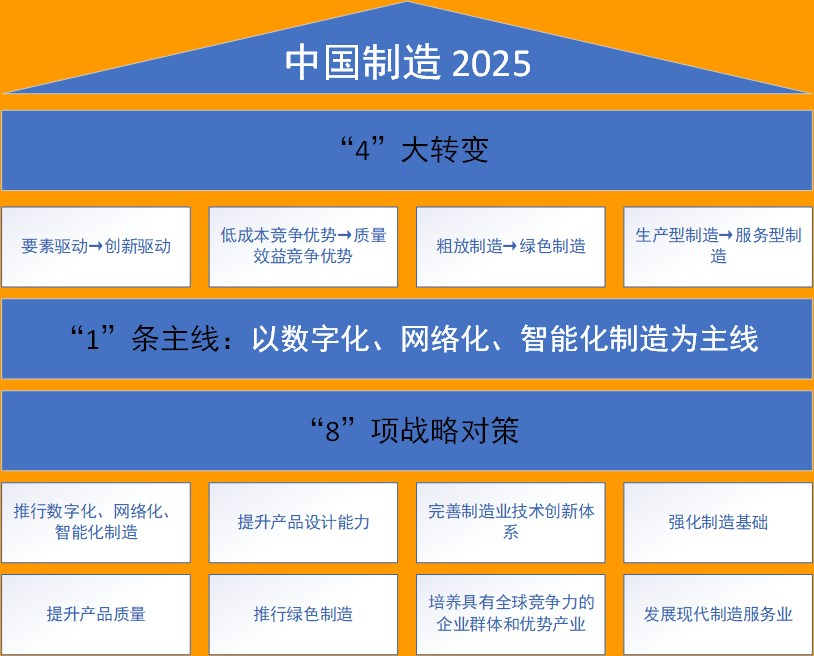
\includegraphics[angle=0,width=10cm]{./figure/4.2.jpg}
\caption{\label{4.2}中国制造2025顶层设计(418模型)}
\end{figure}

《中国制造2025》提出,坚持“创新驱动、质量为先、绿色发展、结构优化、人才为本”的基本方针,坚持“市场主导、政府引导,立足当前、着眼长远,整体推进、重点突破,自主发展、开放合作”的基本原则,通过“三步走”实现制造强国的战略目标:第一步,到2025年迈入制造强国行列;第二步,到2035年我国制造业整体达到世界制造强国阵营中等水平;第三步,到新中国成立约100年时,我国制造业大国地位更加巩固,综合实力进入世界制造强国前列。

围绕实现制造强国的战略目标,《中国制造2025》明确了9项战略任务和重点:一是提高国家制造业创新能力;二是推进信息化与工业化深度融合;三是强化工业基础能力;四是加强质量和品牌建设;五是全面推行绿色制造;六是大力推动重点领域突破发展,聚焦十大重点领域;七是深入推进制造业结构调整;八是积极发展服务型制造和生产型服务业;九是提高制造业国际化发展水平。国务院办公厅关于成立国家制造强国建设领导小组的通知,要求国务院副总理马凯任组长,与来自发改委、财政部、教育部等24个部门的25名部门领导组建领导小组,统筹协调国家制造强国建设全局性工作,审议推动制造业发展的重大规划、重大政策、重大工程专项和重要工作安排等;加强战略谋划,指导各地区、各部门开展工作,协调跨地区、跨部门重要事项,加强对重要事项落实情况的督促检查,采取一切措施推动我国向制造强国挺进。

《中国制造2025》提出,此次制造业转型升级顺应“互联网+”的发展趋势,以信息化与工业化深度融合为主线,重点发展新一代信息技术、高档数控机床和机器人、航空航天装备、海洋工程装备及高技术船舶、先进轨道交通装备、节能与新能源汽车、电力装备、新材料、生物医药及高性能医疗器械、农业机械装备十大领域。

\item 欧盟数字化单一市场
\label{sec:org1904c6f}

在第三次工业革命的浪潮中,为应对能源、环境与可持续发展的挑战,更快、更好地为用户提供高质量产品和高水平服务,并且在与美日以及中印等新兴经济体的竞争中占据先机,欧盟一直高度关注智能制造的发展,并且设立了“智能制造系统”(IMS)、“未来工厂”等多个发展计划,持续投入资金进行相关研究。

《欧洲数字议程》是《欧洲2020战略》的七大旗舰计划之一,于2010年5月由欧盟委员会发布,目的是实现智慧化、可持续和包容性增长。《欧洲数字议程》分析了影响欧盟数字技术发展的七种障碍:数字市场间的堡垒、缺少互操作性、网络犯罪增加与风险、缺少投资、研发与创新不够、社会缺少数字技术知识普及、未能应对社会大的挑战等。针对这些问题,欧盟提出了七个方面的优先行动:1、建立一个新的数字市场,让数字时代的各种优势及时共享;2、改进信息技术领域的标准与互操作性;3、增强网络信任与安全措施;4、增加欧盟对快速和超速互联网的接入;5、加强信息技术的前沿研发与创新;6、加强全体欧洲人的数字技能与可接入的在线服务;7、释放信息技术服务社会的潜能,应对各种社会挑战。建设数字单一市场是《欧洲数字议程》的最核心目标,位居欧盟委员会主席让-克洛德·容克十项优先工作中的第二位。

2015年3月,欧洲宣布了“单一数字市场”战略的优先行动领域,并将发展智能工业作为其中之一。该战略关注3大关键领域:提高数字商品和服务的易用性,培育繁荣数字网络和服务的环境,打造具备长期增长潜力的欧洲数字经济和数字社会。在“打造欧洲数字经济和数字社会”这一关键领域中,欧盟提出了智能工厂、标准、大数据、云计算和数字化技能5个优先行动领域,这实际上将欧盟“未来工厂”战略计划和工业4.0等国家战略相统一。在欧盟对智能制造的推动上,德国始终扮演着最积极的角色,其提出的“工业4.0”已经势不可挡,几乎成为欧洲未来智能制造总体发展构想的代名词。此外,英国也开始思索如何在未来形成更具竞争力的制造业,其标志性成果就是一系列“制造的未来”研究报告。

\begin{figure}[htbp]
\centering
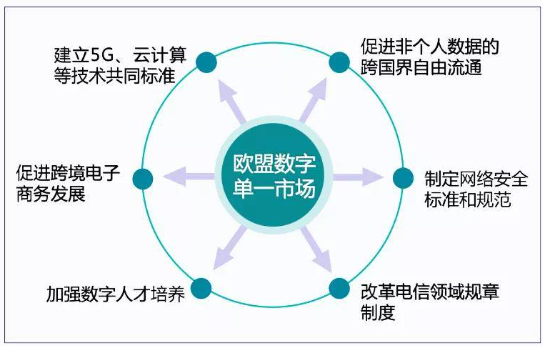
\includegraphics[angle=0,width=10cm]{./figure/4.3.png}
\caption{\label{4.3}欧盟实施“数字单一市场”的主要举措}
\end{figure}


根据2017年5月欧盟委员会发布的数字单一市场战略中期评估报告,欧盟已实现了这份战略中提出的35项法律提案和政策倡议。为推进数字单一市场建设,欧盟委员会还发布了《走向繁荣的数据驱动型经济》、《欧洲工业数字化》、《欧洲网络平台与数字单一市场的机遇与挑战》、《建立欧洲数据经济》等政策文件。

从以欧盟为核心的国际智能制造系统计划来看,欧盟非常关心智能制造的可持续、节能、绿色这些从事实结果来看的方面,以及标准化、教育等方面。但是从欧盟和成员国自身的计划来看,智能工厂和软件密集型嵌入式系统是重点。欧洲的企业对这两个联合研发计划也是格外重视,并且积极投入面向未来智能制造的转型之中,比如西门子、博世等大型工业企业现在也摇身变为IT企业。
\end{enumerate}

\subsection{智能制造应用案例}
\label{sec:org9012b0d}
\begin{enumerate}
\item 西门子数字工厂
\label{sec:orgd08290a}

\setlength{\parindent}{2em}
西门子数控(南京)有限公司(SNC)新工厂近日正式投运,在实地建设之前,西门子就已全面应用自身数字化技术,预先在虚拟世界打造工厂的数字孪生,实现从需求分析、规划设计、动工实施到生产运营全过程的数字化。据介绍,通过打通从研发到生产运营各环节的数据流,新工厂的产能提高近2倍,生产效率提升20\%,产品上市时间缩短近20\%。

SNC成立于1996年,是西门子运动控制领域德国以外最大的研发和制造中心,主要产品线覆盖数控系统、通用变频器、伺服电机、齿轮马达等产品,广泛应用于汽车、航空、电子、制药、物流和新能源等高端制造行业,并有大量产品出口海外市场。面对日益增长的市场需求,该工厂急需扩大产能,提高生产效率和灵活性。于是,催生出再新建一座工厂的需要。

何为原生数字化工厂?西门子全球执行副总裁,西门子中国董事长、总裁兼首席执行官肖松表示,原生指的是在设计、规划、建造和生产运营的全生命周期,从零开始,开创性地完全使用西门子自身的数字化理念和技术,让工厂从无到有,由虚到实。“在工厂破土动工之前,已经在虚拟世界里用西门子的软件,完成了从工厂需求、分析到建成、运营全过程模拟仿真和验证。在实际建设过程中,通过大数据分析,进一步优化生产流程,为实际生产提供实时可靠的数据支撑,实现数字化制造和管理。”

\begin{figure}[htbp]
\centering
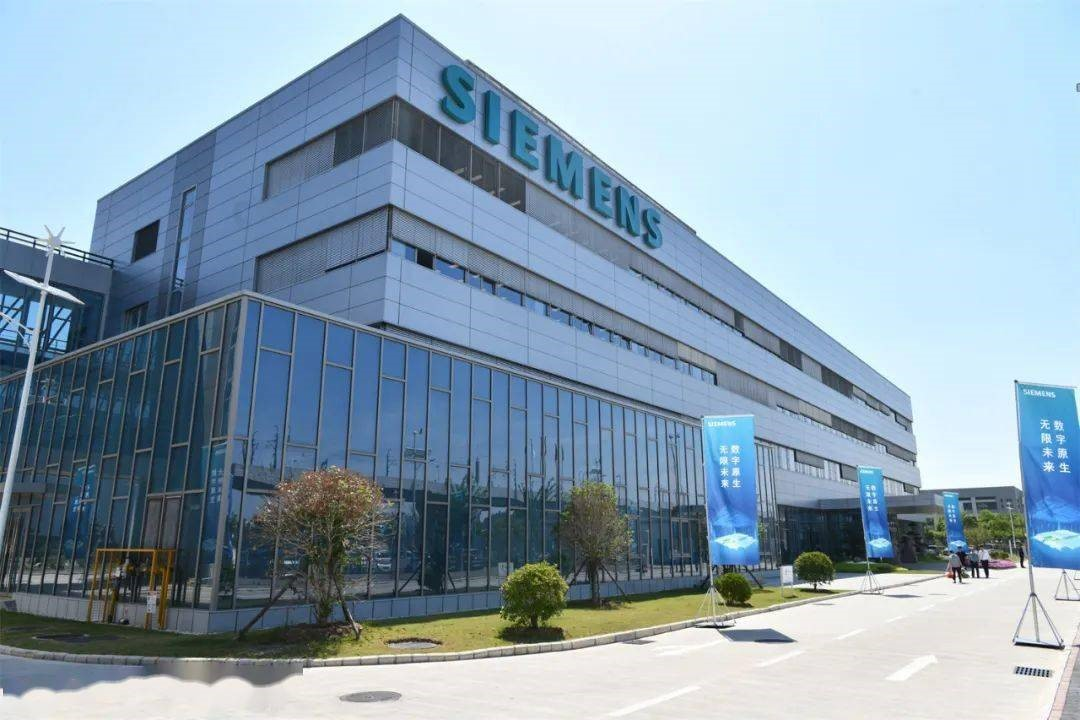
\includegraphics[angle=0,width=10cm]{./figure/4.4.jpg}
\caption{\label{4.4}西门子原生数字化工厂}
\end{figure}


新工厂在实体建设及运营阶段,基于西门子工业云的大数据分析及其与工业物联网系统的有机结合,进一步优化生产流程,为实际生产提供实时数据支撑,实现数字制造和管理。新工厂可同时生产电子和电机制造两大类从原材料、生产设备到工艺流程均截然不同的产品。

数据和数字化也是创造高度可持续性生产环境的基础。通过打造该工厂的数字孪生,可以节省资源和材料,从而在施工开始之前就降低了场地对环境的影响。

根据西门子雄心勃勃的可持续发展框架DEGREE,新工厂还配备了自动LED照明、高效泵、风扇和冷却元件,所有这些将让工厂每年节省超过500万千瓦时的电力。该工厂还安装了光伏系统,每年可减少3300吨碳排放,相当于在慕尼黑和纽约之间往返400趟航班。集成的雨水回收系统每年节约用水量达到6000立方米。

\item GE航空
\label{sec:org925a1d2}

作为世界上最大的多元化工业集团,GE公司提出了“工业互联网”构想,将工业革命与互联网革命统一为“第三波”创新与变革,有人将其与德国工业4.0相提并论,认为其代表了美国的智能制造变革。智能设备、智能系统、智能决策以及三者的集成是“工业互联网”三大数字元素,虽然一家公司不可能完全代表美国智能制造的发展方向,但其明确的“智能化”理念依然是新一轮变革中的鲜明主题。

GE公司认为“工业互联网”是两大革命中先进技术、产品与平台的结合,即工业革命中的机器、设施与网络和互联网革命中的计算、信息、通信结合\cite{Evans2012}。“工业互联网”将通过智能机床、先进分析方法以及人的连接,使数字世界与机器世界深度融合,深刻改变全球工业。从创造价值的角度来看,GE公司认为“工业互联网”的价值可以从三方面体现:第一,提高能源的使用效率;第二,提高工业系统与设备的维修和修护效率;第三,优化并简化运营,提高运营效率。

“智能”是“工业互联网”的关键词(见图\ref{4.5}),GE公司正在飞机发动机上诠释“智能”的概念。飞机发动机上的各种传感器会收集发动机在空中飞行时的各种数据,将这些数据传输到地面,经过智能软件系统分析,可以精确地检测发动机的运行状况,甚至预测故障,进行预先维修提示等,以提升飞行安全性和发动机的使用寿命。

\begin{figure}[htbp]
\centering
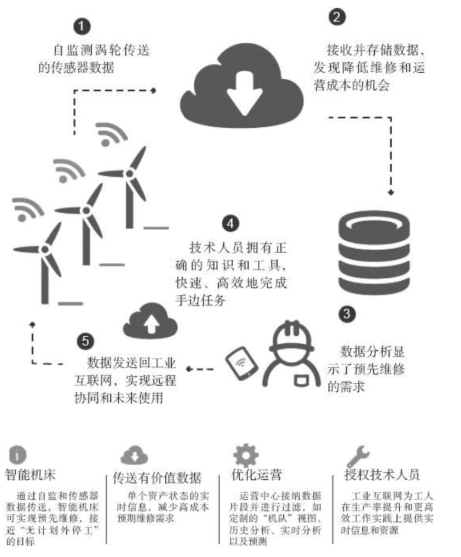
\includegraphics[angle=0,width=7cm]{./figure/4.5.png}
\caption{\label{4.5}工业互联网的“智能”}
\end{figure}


\item 德国奔驰
\label{sec:org5916215}

奔驰公司的历史可以追溯到1883年奔驰汽车公司成立,是人类历史上的第一个汽车品牌。1926 年奔驰汽车厂和戴姆勒汽车厂合并成立戴姆勒-奔驰汽车公司,正式推出享誉世界的“梅赛德斯-奔驰”品牌,1998年并购美国克莱斯勒汽车公司,更名为现在的“戴姆勒 - 克莱斯勒”。

奔驰位于德国辛德芬根的56号汽车工厂(Factory 56),是奔驰按照工业4.0标准打造的未来工厂,以“数字化、柔性化、绿色化”为核心目标。工厂里物料传输、机械臂等自动化智能生产应用非常瞩目,不同结构的汽车可在56号工厂同一装配线生产,生产设备可与它周围的部件及汽车进行互联互通,同时无人运输系统保证了灵活性。

56号工厂实现了梅赛德斯-奔驰汽车的智能生产愿景。所有数字化活动的核心是MO360数字生态系统,该系统在56工厂首次得到充分利用。MO360包括一系列通过共享接口和标准化用户界面连接的软件应用程序,使用实时数据支持全球梅赛德斯-奔驰汽车的生产。MO360整合了全球30多家奔驰汽车工厂的主要生产流程和IT系统的信息,汇集了重要的软件应用。例如,它提供了显著优化的基于KPI的生产控制。它还使每个员工都能实时获得基于需求的个人信息和工作说明。MO360的主要成分已经在全球30多家工厂使用。MO360在一个功能单元中结合了效率和质量工具,在高度数字化的汽车生产中实现了最大的透明度。

\begin{figure}[htbp]
\centering
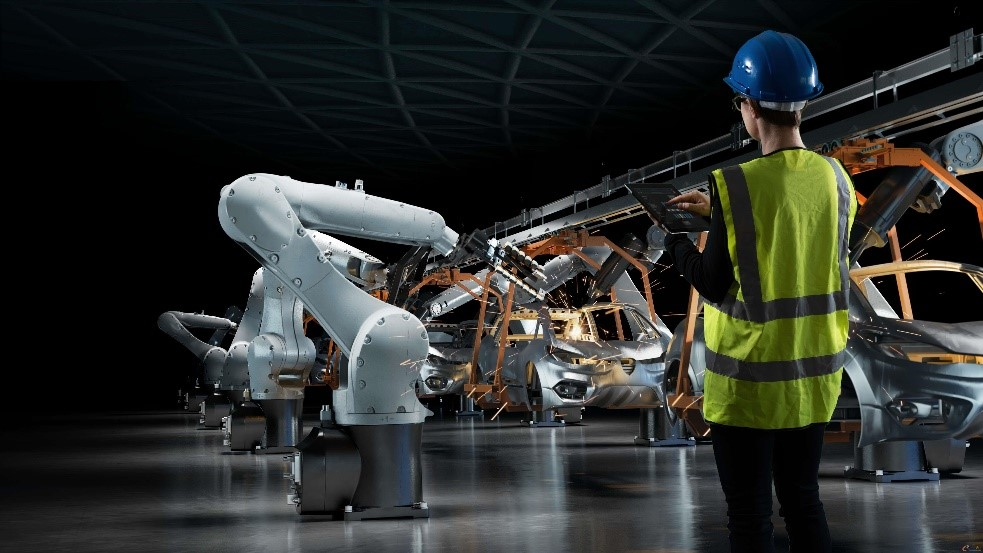
\includegraphics[angle=0,width=10cm]{./figure/4.6.jpg}
\caption{\label{4.6}奔驰56号汽车工厂}
\end{figure}


在56号工厂,新的数字基础设施配备了高性能WLAN和5G网络,为全面数字化提供了重要基础。它使用超现代工业4.0应用程序,从智能设备到大数据算法。数字生产技术已在各地得到应用。此外,56号工厂完全无纸化:由于通过定位系统对生产线上的每辆车进行数字跟踪,与员工相关的车辆数据通过数字设备和显示屏实时显示在生产线上。总而言之,这将每年节省大约10吨纸。

机器和生产设备在整个工厂都是相互连接的;其中大多数已经具备物联网(IoT)能力。这种360度的连接不仅延伸到56号工厂本身,而且还超越了设施,延伸到整个价值链:在56号工厂的开发和规划过程中,已经使用了虚拟或增强现实等数字技术,而且有助于提高批量生产的灵活性和效率。在与供应商和运输服务提供商的对话中,还利用了跟踪和追踪的好处,使物流能够在世界各地进行数字追踪。


\item 中国海尔
\label{sec:orgb7dd426}

2022年3月30日,世界经济论坛在瑞士日内瓦公布了第八批全球灯塔工厂名单,此次共有13座“数字化制造”和“全球化4.0”示范者入选,其中包括郑州海尔热水器互联工厂,这是全球热水器行业首座端到端灯塔工厂,也是海尔继胶州中央空调、沈阳冰箱、天津洗衣机之后的第4座端到端灯塔工厂。

“灯塔工厂”被称为“世界上最先进的工厂”,由达沃斯世界经济论坛和麦肯锡咨询公司共同遴选,是全球智能制造领域的风向标。郑州海尔热水器互联工厂的入选,让海尔分别在空调、冰箱、洗衣机、热水器4大产业打造出行业的首个灯塔工厂,成为国内拥有灯塔工厂数量最多的企业之一,持续引领中国智能制造走在世界前列。

在中国制造2025战略指引下,海尔逐步探索出一条以互联工厂为核心的智能制造发展路线。从2005年开始,提出要把传统制造变成大规模定制。2008年,对整个企业的产品制造体系进行了模块化改造,同时在虚拟设计、实体制造方面进行了系统的建设。从模块化到自动化再到黑灯工厂的建设,到建成互联工厂,不断持续的试错。

海尔理解的互联工厂不是一个工厂的转型,而是一个生态系统,整个企业全系统全流程都要进行颠覆,通过互联使用户获得最佳体验,在满足用户个性化需求的同时给企业创造效益。满足用户个性化需求是前提,然后才可以通过高效率实现企业的高收益。

\begin{figure}[htbp]
\centering
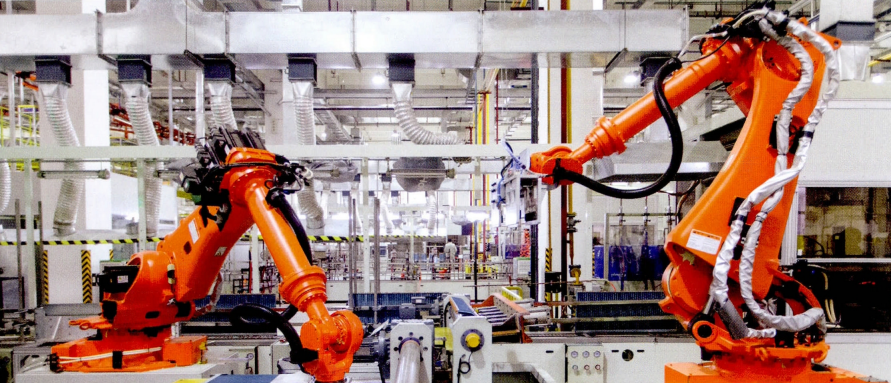
\includegraphics[angle=0,width=10cm]{./figure/4.7.png}
\caption{\label{4.7}海尔的互联工厂}
\end{figure}

海尔打造的互联工厂不是一个物理空间,或者传统意义上的车间,而是一个用户交互的网络空间,一个虚拟和实体交融的空间。因此,海尔互联工厂进行了第三个颠覆,即由过去封闭、博弈、不可持续的企业关系,颠覆为一切是以用户需求为驱动的共创共赢生态圈\cite{邓雅静2017}。在海尔生态圈里,有小微、员工、创客、资源、供应商、设备商、营销商、消费者、媒体等。每个环节都是生态圈中的一环。“在生态圈里,海尔和创客、小微、供应商的合作模式与原来也有本质区别。比如,供应商原来是按照图纸、订单为海尔来供货。现在,海尔生态圈把供应商和用户连接起来,把供应商和互联工厂的所有环节连接起来。在这种情况下,供应商的方案如果被用户选择,就可以获取订单,如果不被选择则被淘汰。同时,供应商一旦被用户选择,他的订单会愈来愈多,分享的价值就越来越大,积极性就越来越高,随之供应的零部件的质量、效率也就越来越高,实现了各有关方利益最大化。”

从2015年海尔第一个互联工厂——沈阳冰箱互联工厂投产至今,海尔已经建成数个互联工厂。值得一提的是,建设互联工厂的丰富经验,已经被海尔提炼成自己的方法——COSMO平台。这个平台可以把海尔互联工厂的模式产品化。”海尔家电集团副总裁、供应链总经理陈录城介绍说。


\printbibliography[heading=bibintoc,title=参考文献]
\end{enumerate}
\end{document}